\chapter{Guaranteed Escape Speed}
\label{chap:nonconservative}
\graphicspath{{Results/Images/}}

In this chapter, we will discuss the results from the non-conservative guaranteed escape speed analytical method developed in \Cref{sec:escape_speed_derivation}. The algorithm's absolute performance and its viability is discussed and compared with that of the conservative guaranteed escape speed algorithm.

\section{Simulation Setup}
\label{sec:nonconservative_simulation_setup}
As mentioned in \Cref{sec:escape_speed_derivation}, the launch location for testing out the algorithm was chosen to be the longest edge of the ellipsoid shaped asteroid since it helped in simplifying the computation. In addition to this, the particles were launched in the equatorial plane such that the orbital inclination remained zero \footnote{The orbital inclination remains zero valued after the launch in a non-uniform gravity field because the central body is homogeneous as well as symmetrical about the equator which means that there is equal attraction in the positive and negative z-axis directions which cancel each other out.}, which further simplified the computation.
%
\newline\newline
%
We compare the results from our derivation of the non-conservative guaranteed escape speed with that of the conservative approach as defined by \cite{scheeresBook}. To use the algorithm, the following launch conditions were used (these launch conditions are also depicted in \Cref{fig:non_conservative_launch_vectors}):
%%%
\begin{enumerate}
    \item The launch location is at the longest edge of the ellipsoid.
    \item The launch azimuth is equal to \SI{270}{\degree}.
    \item The launch declinations are varied from \SI{10}{\degree} to \SI{80}{\degree}.
    \item The launch velocity was kept fixed and chosen at random to be \SI{6.0}{\metre \per \second}
\end{enumerate}
%%%
Note that these launch conditions result in equatorial orbits, just like how we want to test the non-conservative escape speed algorithm. The value for the parameter $q_\infty$ in \Cref{eqn:non_conservative_inertial_guaranteed_escape_speed}, which is the periapsis distance for a parabolic escape trajectory, was set manually for each simulated trajectory and remained constant during the entire duration of each simulation. Several values of $q_\infty$ were used for testing and they were all taken as fractions of the largest dimension of the ellipsoid. This was done because we do not yet have a dedicated process to determine the value of $q_\infty$ and hence several random fractions were used to guage the output.
% Note that $q_\infty$ is the distance from the focus to the vertex of a parabola so in this case it is the distance between the centre of the asteroid and the periapsis distance on the final parabolic escape trajectory. We say \emph{final} because the non-conservative guaranteed escape speed was designed to account for regolith cases that do not immediately lead to an escape scenario after being lofted from the surface of an asteroid but rather take one or more orbital revolutions around the asteroid before embarking on the parabolic escape trajectory. We will witness such a case shortly.
%%%
\begin{figure}[htb]
\centering
\captionsetup{justification=centering}
\subfloat[]{
    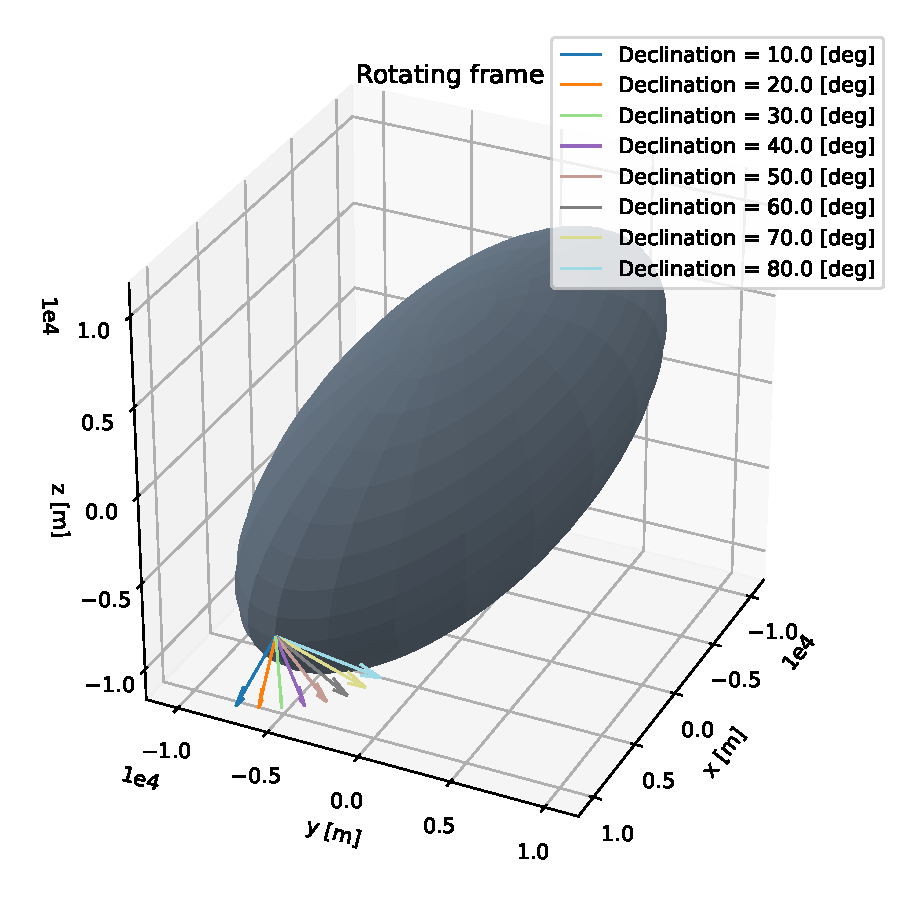
\includegraphics[width=\textwidth, height=0.5\textheight, keepaspectratio=true]{non_conservative_escape_speed/launch_vectors_body_frame.pdf}
    \label{fig:non_conservative_launch_vectors_arf}
}

\subfloat[]{
    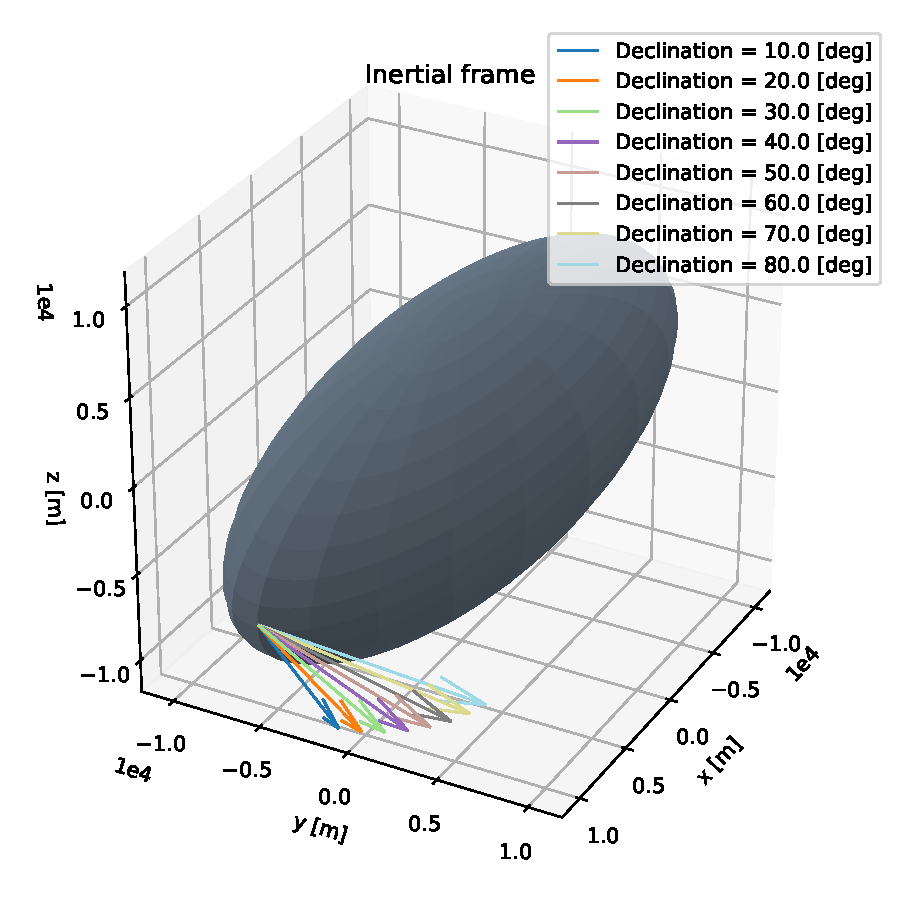
\includegraphics[width=\textwidth, height=0.5\textheight, keepaspectratio=true]{non_conservative_escape_speed/launch_vectors_inertial_frame.pdf}
    \label{fig:non_conservative_launch_vectors_aif}
}
\caption{Launch vectors used for testing the non-conservative escape speed algorithm. \protect\Cref{fig:non_conservative_launch_vectors_arf} shows the vectors expressed in \gls{ARF} and \protect\Cref{fig:non_conservative_launch_vectors_aif} shows the vectors expressed in \gls{AIF}.}
\label{fig:non_conservative_launch_vectors}
\end{figure}
\FloatBarrier
%%%

\section{Conservative Approach With Spherical Asteroid}
\label{sec:conservative_spherical_asteroid_results}
We will first look at the case of a homogeneous spherical asteroid whose radius is equal to the largest semi-major axis of the \gls{CDE} i.e. \SI{20}{\kilo\metre}. The simulation involved launching particles at a constant declination of \SI{45}{\degree} and for launch azimuth varying in the range [0, 360)\si{\degree}. The launch velocities ranged from 1 - \SI{20}{\metre \per \second} and the simulations did not include perturbations, gravity or otherwise. We used the \gls{CDE} potential model but all three semi-major axes were made equal to \SI{20}{\kilo\metre}. In such a case, the \gls{CDE} gravity potential model acts like a point mass potential model. This situation works for us since the latter is the actual gravity potential model for a point external to a homogeneous spherical body \parencite{macmillanPotential}.
%%%
\begin{figure}[htb]
\centering
\captionsetup{justification=centering}
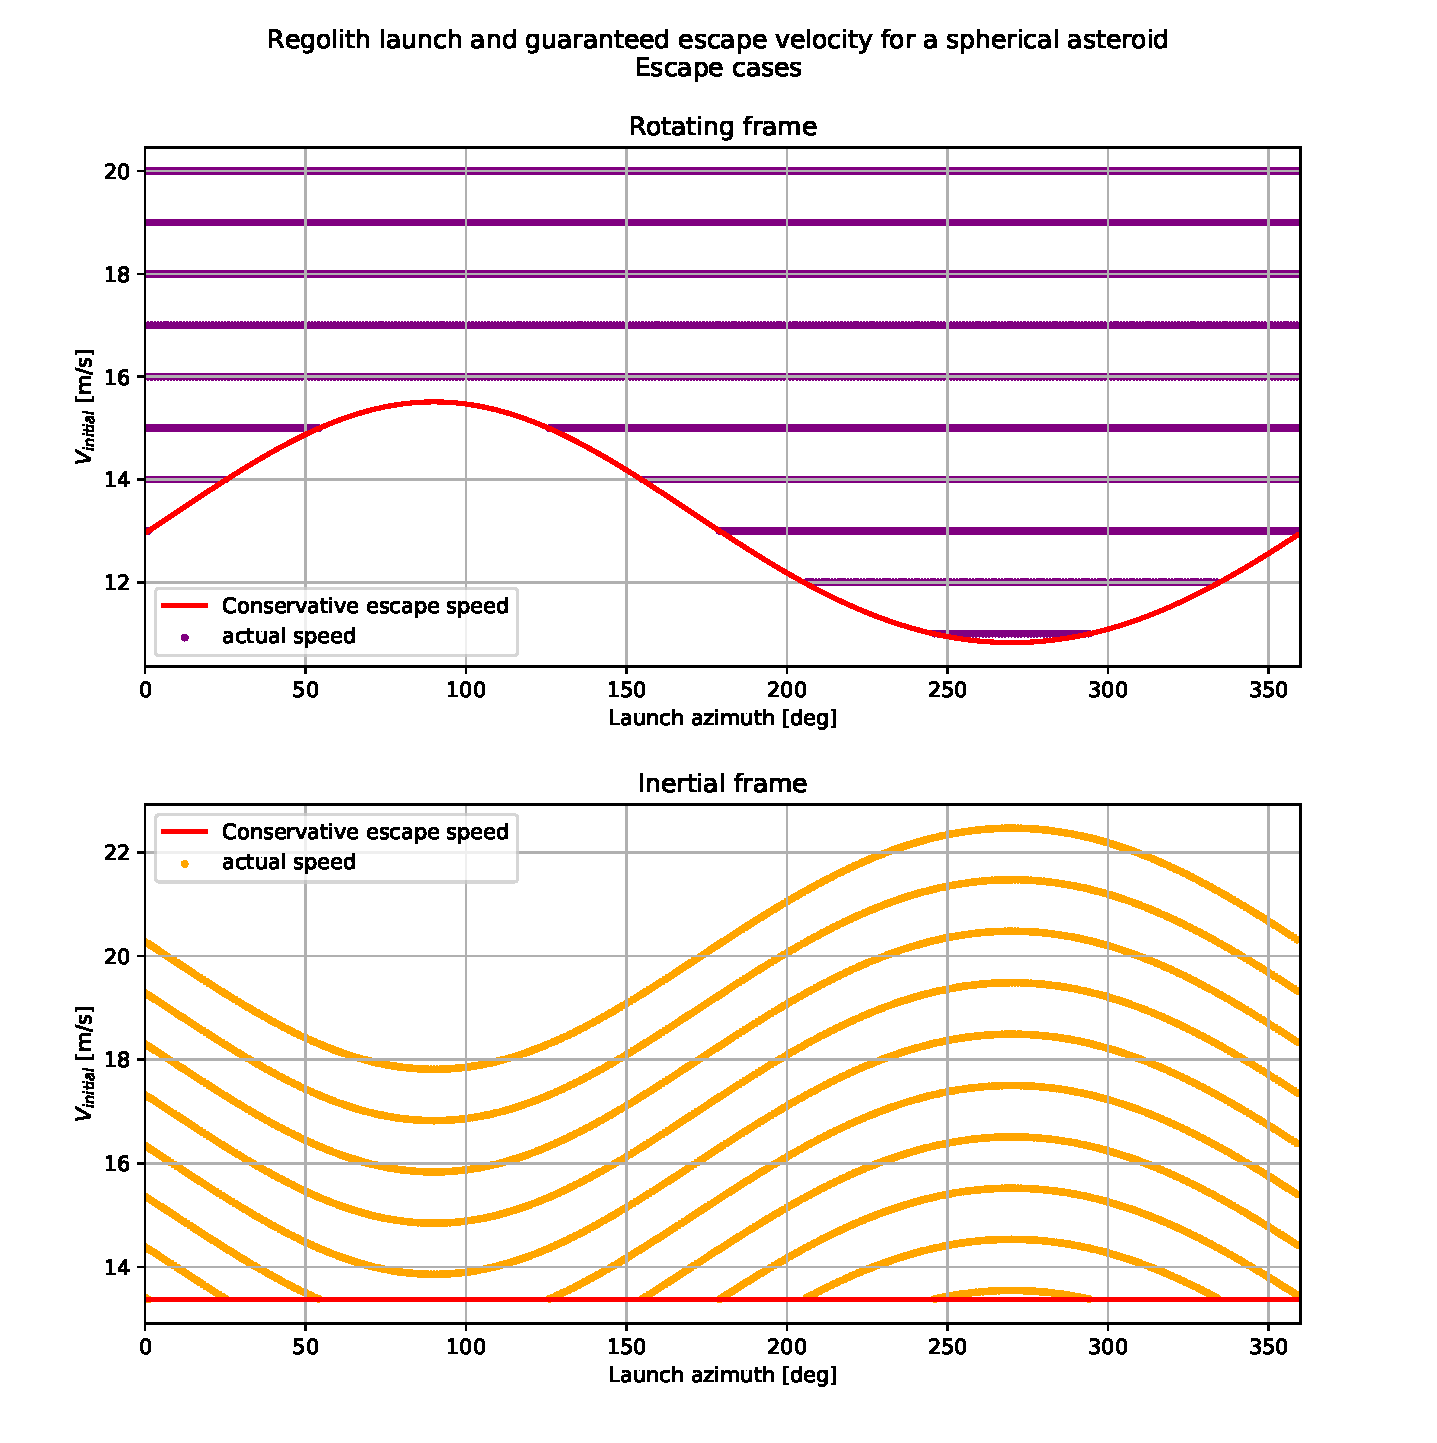
\includegraphics[width=\textwidth, height=0.7\textheight, keepaspectratio=true]{non_conservative_escape_speed/spherical_asteroid_conservative_escape_speed.pdf}
\caption{Escape velocities for varying launch azimuths and a constant launch declination of \protect\SI{45}{\degree}. The conservative guaranteed escape speed curve clearly separates all escape scenarios, as shown in both \protect\gls{AIF} and \protect\gls{ARF}.}
\label{fig:conservative_spherical_asteroid_escape}
\end{figure}
\FloatBarrier
%%%
The algorithm for the conservative guaranteed escape speed works properly for the case of a homogeneous spherical asteroid, as shown in \Cref{fig:conservative_spherical_asteroid_escape}, whose gravity potential is equivalent to that of a point mass. An escape occurs only if the particle was launched with a velocity which is equal to or above the conservative guaranteed escape speed curve and not otherwise. \Cref{fig:conservative_spherical_asteroid_escape_and_reimpact} shows how the curve even separates out all the re-impact cases. All launch velocities that are below the escape speed curve result only in re-impact and nothing else. Note that for this particular simulation we did not obtain any capture cases, but only escape and re-impact.
%%%
\begin{figure}[htb]
\centering
\captionsetup{justification=centering}
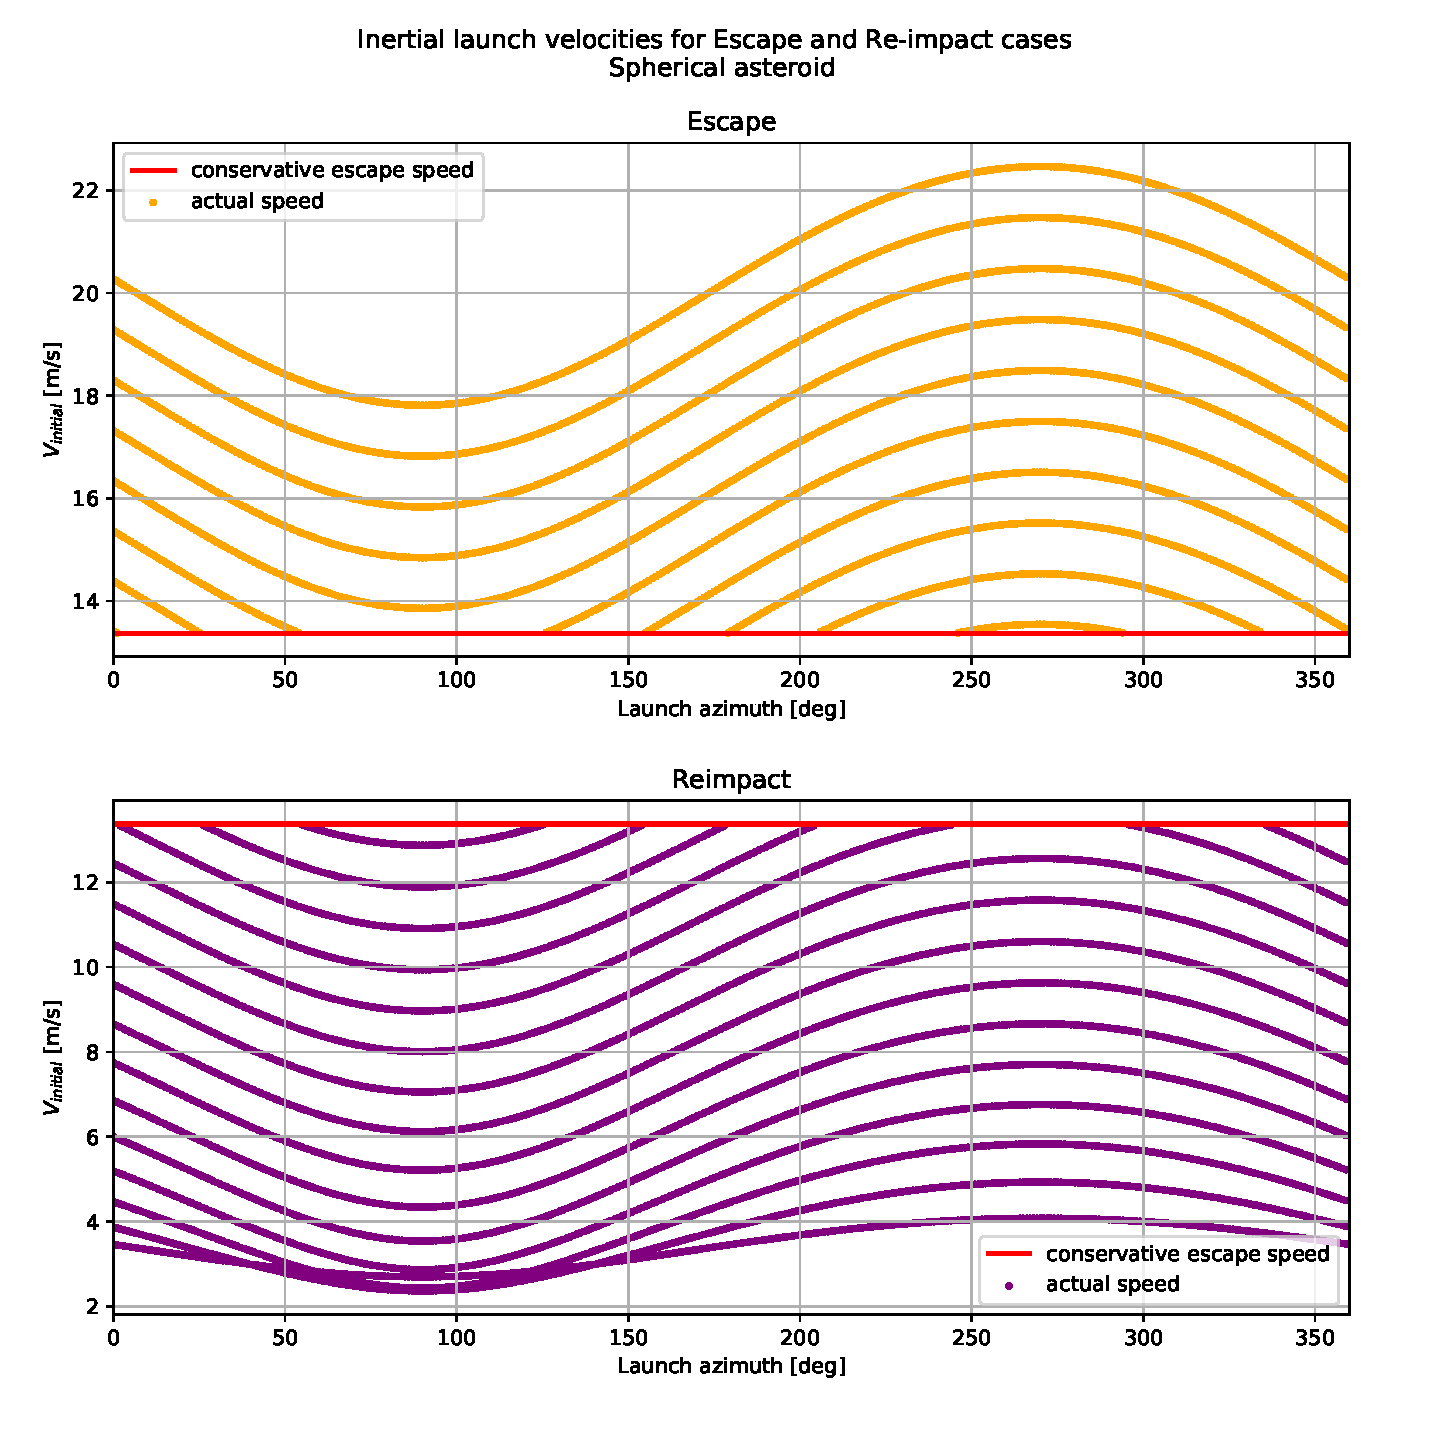
\includegraphics[width=\textwidth, height=0.7\textheight, keepaspectratio=true]{non_conservative_escape_speed/spherical_asteroid_escape_and_capture.pdf}
\caption{Escape and re-impact scenario velocities for varying launch azimuths and a constant launch declination of \protect\SI{45}{\degree}. The conservative guaranteed escape speed curve clearly separates all re-impact cases from the escape ones.}
\label{fig:conservative_spherical_asteroid_escape_and_reimpact}
\end{figure}
\FloatBarrier
%%%

\section{Non-Conservative Approach With Ellipsoidal Asteroid}
\label{sec:nonconservative_escape_cde_results}
Now we shall look at the results for a \gls{CDE} model, for which a particle was launched with the initial conditions enlisted earlier. \Cref{fig:non_conservative_escape_multiple_qinfinity_single_velocity} shows the inadequacy of the conservative guaranteed escape speed algorithm to predetermine escape scenarios based just on the initial conditions, as it fails to account for escape situations that occur at lower declination angles. However, for all launch velocities above the conservative escape speed curve, we only witness escape scenarios which is how it should be and any result contrary to this means the simulator is at fault. The non-conservative escape speed algorithm, does not function as expected. The algorithm was designed, hoping that it would also account for escape cases that the conservative approach was unable to. \Cref{fig:non_conservative_escape_multiple_qinfinity_single_velocity} shows the non-conservative escape speed curves for three different $q_\infty$ values and although we get an idea on the performance from individual $q_\infty$ values, the algorithm in general fails to identify escape scenarios since there are cases (at higher declination angles) where the launch velocity lies below the $q_\infty$ curves but belongs to the escape regime.
%%%
\begin{figure}[htb]
\centering
\captionsetup{justification=centering}
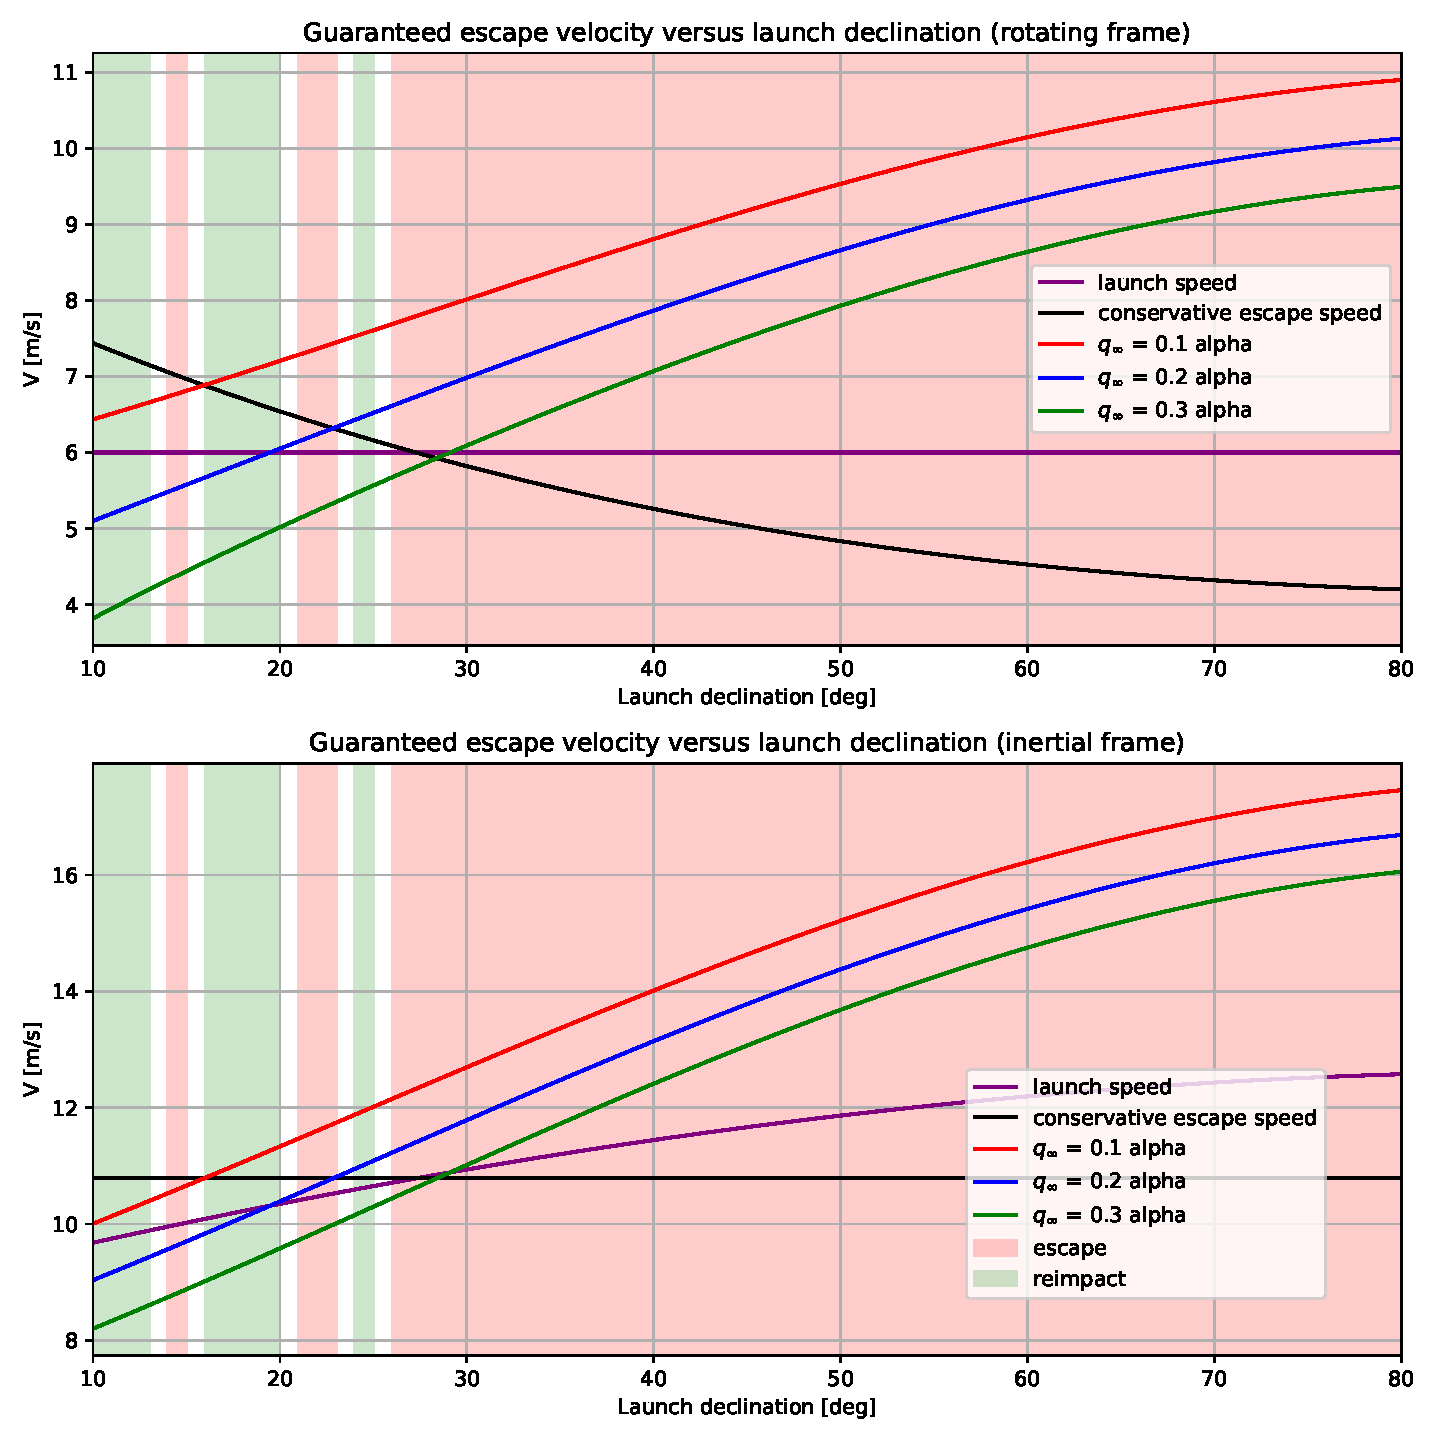
\includegraphics[width=\textwidth, height=0.7\textheight, keepaspectratio=true]{non_conservative_escape_speed/multiple_qinfinity_plus.pdf}
\caption{Escape and re-impact scenarios depicted for regolith launched with a single velocity and launch azimuth but multiple launch declination values. Non-conservative escape speed curve is shown for a \gls{CDE} asteroid for three $q_\infty$ values that are fractions of the largest semi-major axes, $\alpha$, of the ellipsoid. The conservative guaranteed escape speed curve is also shown for comparison.}
\label{fig:non_conservative_escape_multiple_qinfinity_single_velocity}
\end{figure}
\FloatBarrier
%%%
It is important to note that in \Cref{fig:non_conservative_escape_multiple_qinfinity_single_velocity}, the non-conservative escape speed curves used only the \emph{"+"} sign part of the formula in \Cref{eqn:non_conservative_inertial_guaranteed_escape_speed} and not the \emph{"-"} sign part since the latter always gave negative velocities for multiple sample values of $q_\infty$. We performed the simulation for the non-conservative approach for the same launch azimuth and range of declination angles as before but velocities ranging from 1 to \SI{16}{\metre \per \second} and $q_\infty=0.3$ to see if the curve provides better escape estimates at other launch velocities. The result of this is shown in \Cref{fig:non_conservative_multiple_velocities_qinfinity_0.3}. We see yet again the failure of the so called non-conservative escape speed algorithm. We witness that even when the launch velocity is above the non-conservative escape speed curve, we have re-impact scenarios. This clearly means that the algorithm is not even able to demarcate re-impact situations. Atleast with the conservative escape speed curve, we know that if the launch velocity is above the curve then the regolith can only escape and not have any other final fate.
%%%
\begin{figure}[htb]
\centering
\captionsetup{justification=centering}
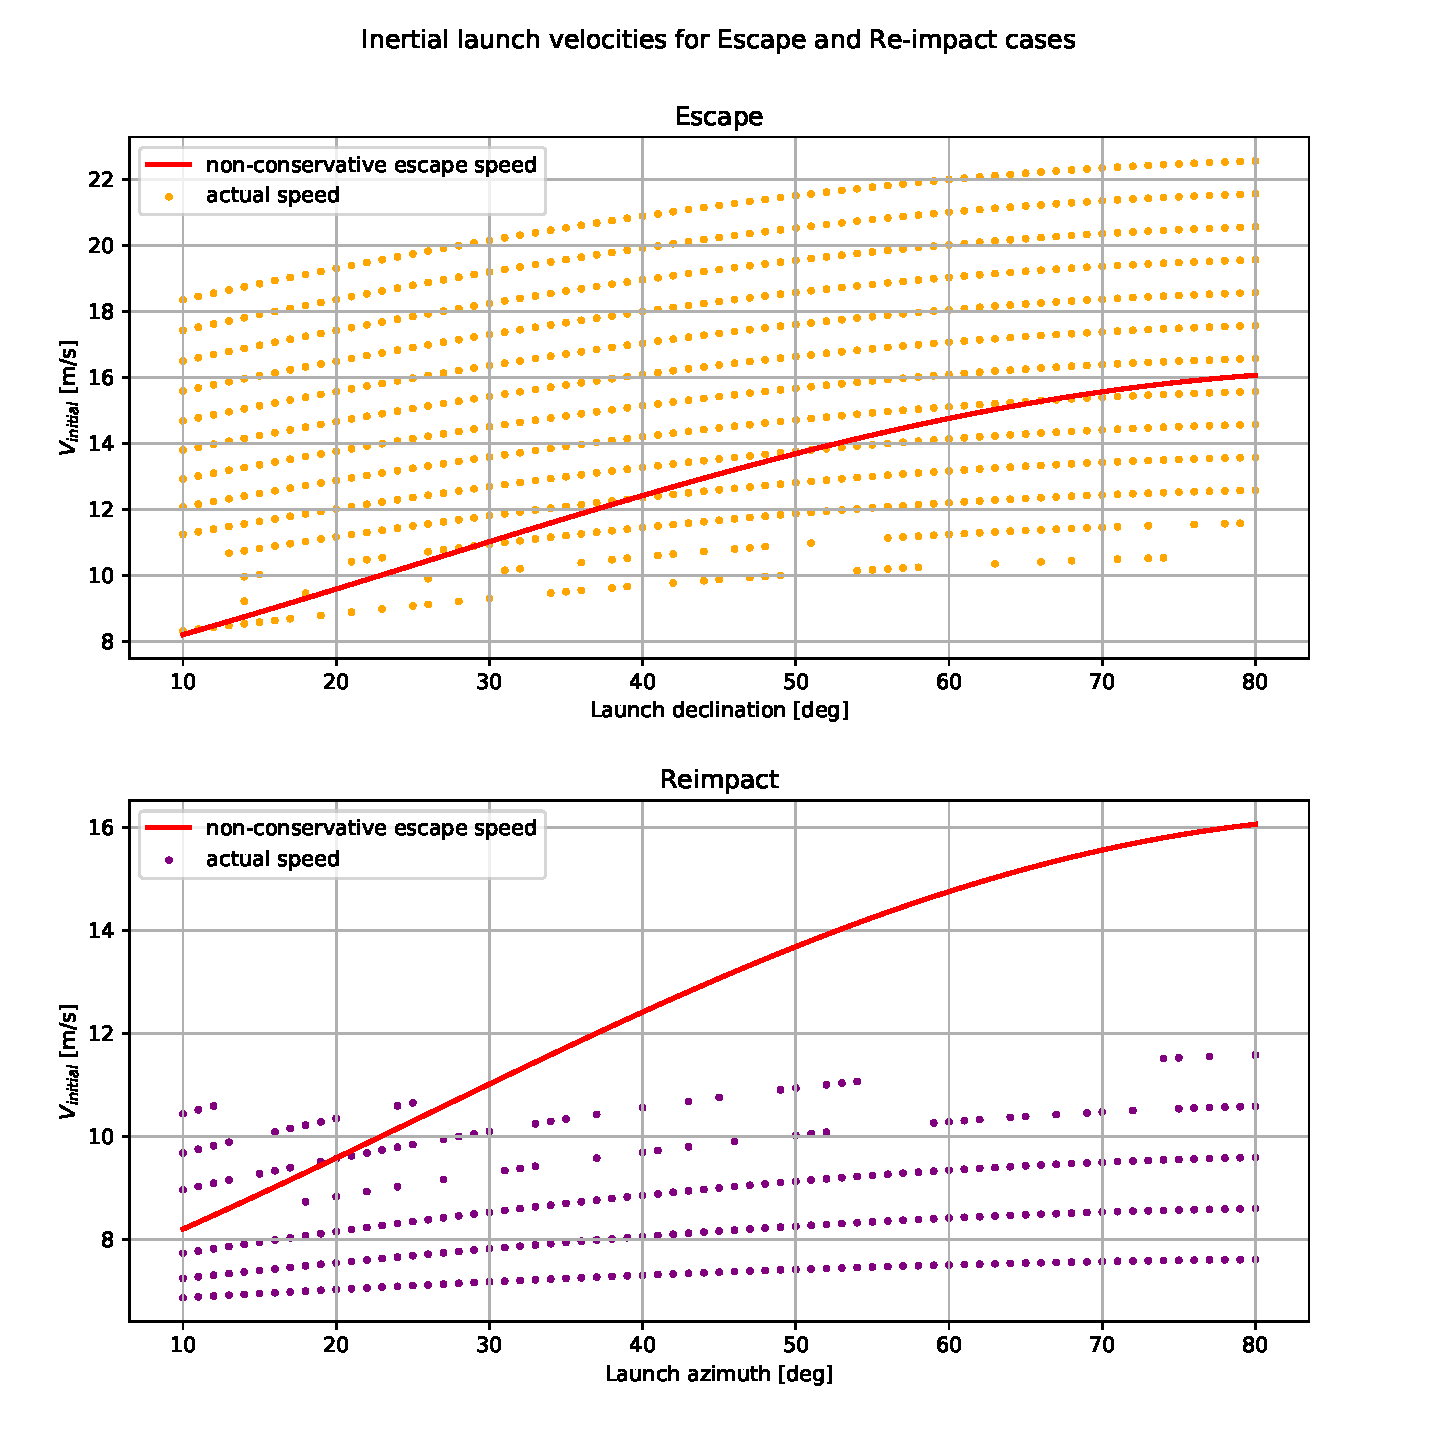
\includegraphics[width=\textwidth, height=0.7\textheight, keepaspectratio=true]{non_conservative_escape_speed/qinfinity_dot3_escape_reimpact_multipleVelocities.pdf}
\caption{Escape and re-impact scenarios depicted for regolith launched from the longest edge of \gls{CDE} with multiple velocities with launch azimuth = \SI{270}{\degree} and launch declination in the range of 10 to \SI{80}{\degree}. The non-conservative escape speed curve is shown for $q_\infty = 0.3$.}
\label{fig:non_conservative_multiple_velocities_qinfinity_0.3}
\end{figure}
\FloatBarrier
%%%
On the other end of the spectrum, we can see that there are launch velocities below the non-conservative escape speed curve where escape scenarios occur. This is another indication of the failure of the algorithm we designed.
%
\newline\newline
%
The other problem with the algorithm is that if we reduce the value of $q_\infty$ beyond certain extent, then we obtain a gibberish curve for the non-conservative escape speed in the \gls{ARF}. An example of this is depicted in \Cref{fig:non_conservative_qinfinity_0.7} where $q_\infty = 0.7$. The curve as expressed in the \gls{ARF} has no meaning since negative speeds are not valid.
%%%
\begin{figure}[htb]
\centering
\captionsetup{justification=centering}
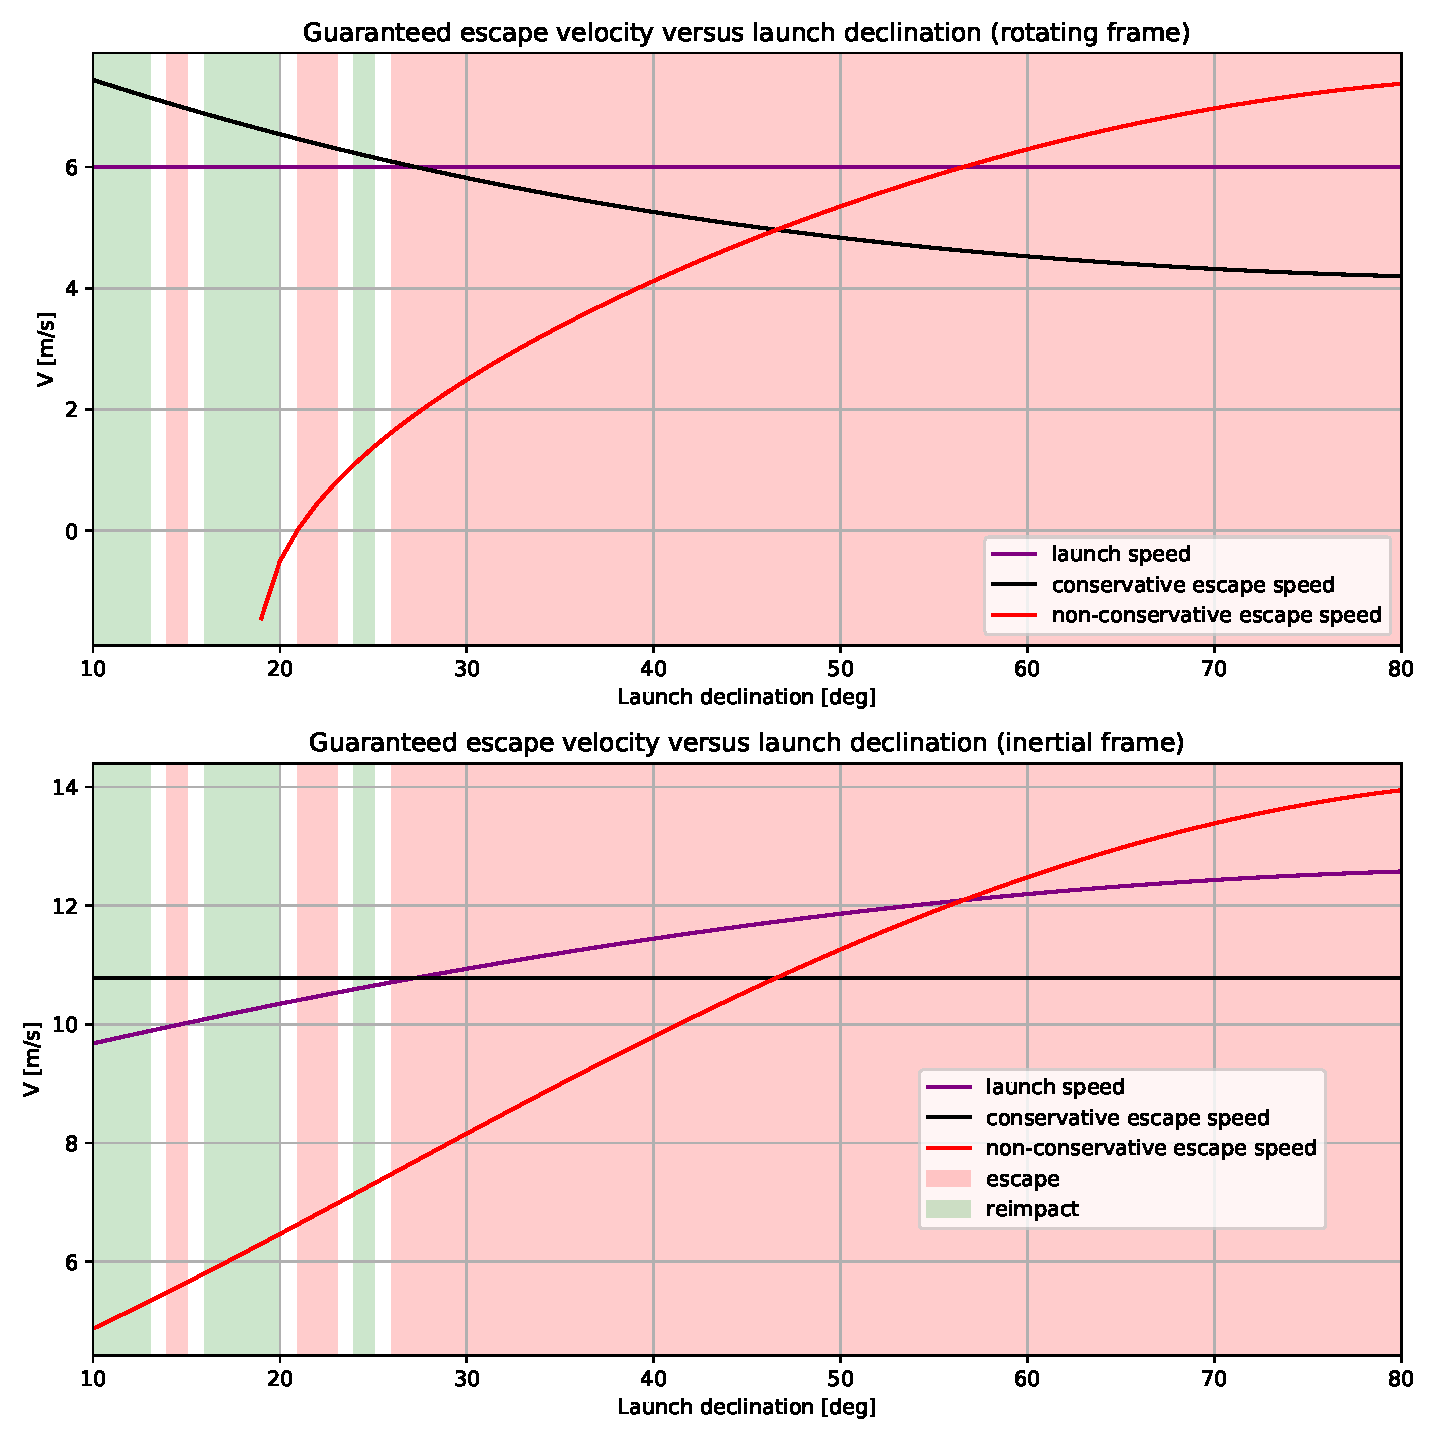
\includegraphics[width=\textwidth, height=0.6\textheight, keepaspectratio=true]{non_conservative_escape_speed/qinfinity_dot7alpha_plus.pdf}
\caption{A non-applicable non-conservative escape speed curve for $q_\infty=0.7$. The curve in the rotating frame or the \gls{ARF} shows negative speed values which is not valid.}
\label{fig:non_conservative_qinfinity_0.7}
\end{figure}
\FloatBarrier
%%%
The non-conservative guaranteed escape speed method did not work as expected in identifying the escape cases that were undetected by the conservative method. In addition to this, we saw that the method produces a valid escape velocity curve only for a small range of $q_\infty$ values. Although the non-conservative method failed, the approach to derive it was correct and now we know that even if it sounds reasonable in theory, it fails completely in practice.

\section{Conservative Approach Limitations With Ellipsoidal Asteroid}
\label{sec:conservative_escape_cde_limitations}
The conservative escape speed approach didn't account for a few escape scenarios when regolith was launched from the surface of a \gls{CDE} shaped asteroid and the reason for that is the combined effect of the shape/gravity field variations and a rapid rotation rate of the asteroid. For example, from the trajectory for the regolith launched at declination angle of \SI{15}{\degree} in \Cref{fig:non_conservative_escape_multiple_qinfinity_single_velocity}, it was observed that the particle completes one revolution around the asteroid before embarking on a final hyperbolic trajectory. This is shown in \Cref{fig:3d_traj_declination_15}.
%%%
\begin{figure}[htb]
\centering
\captionsetup{justification=centering}
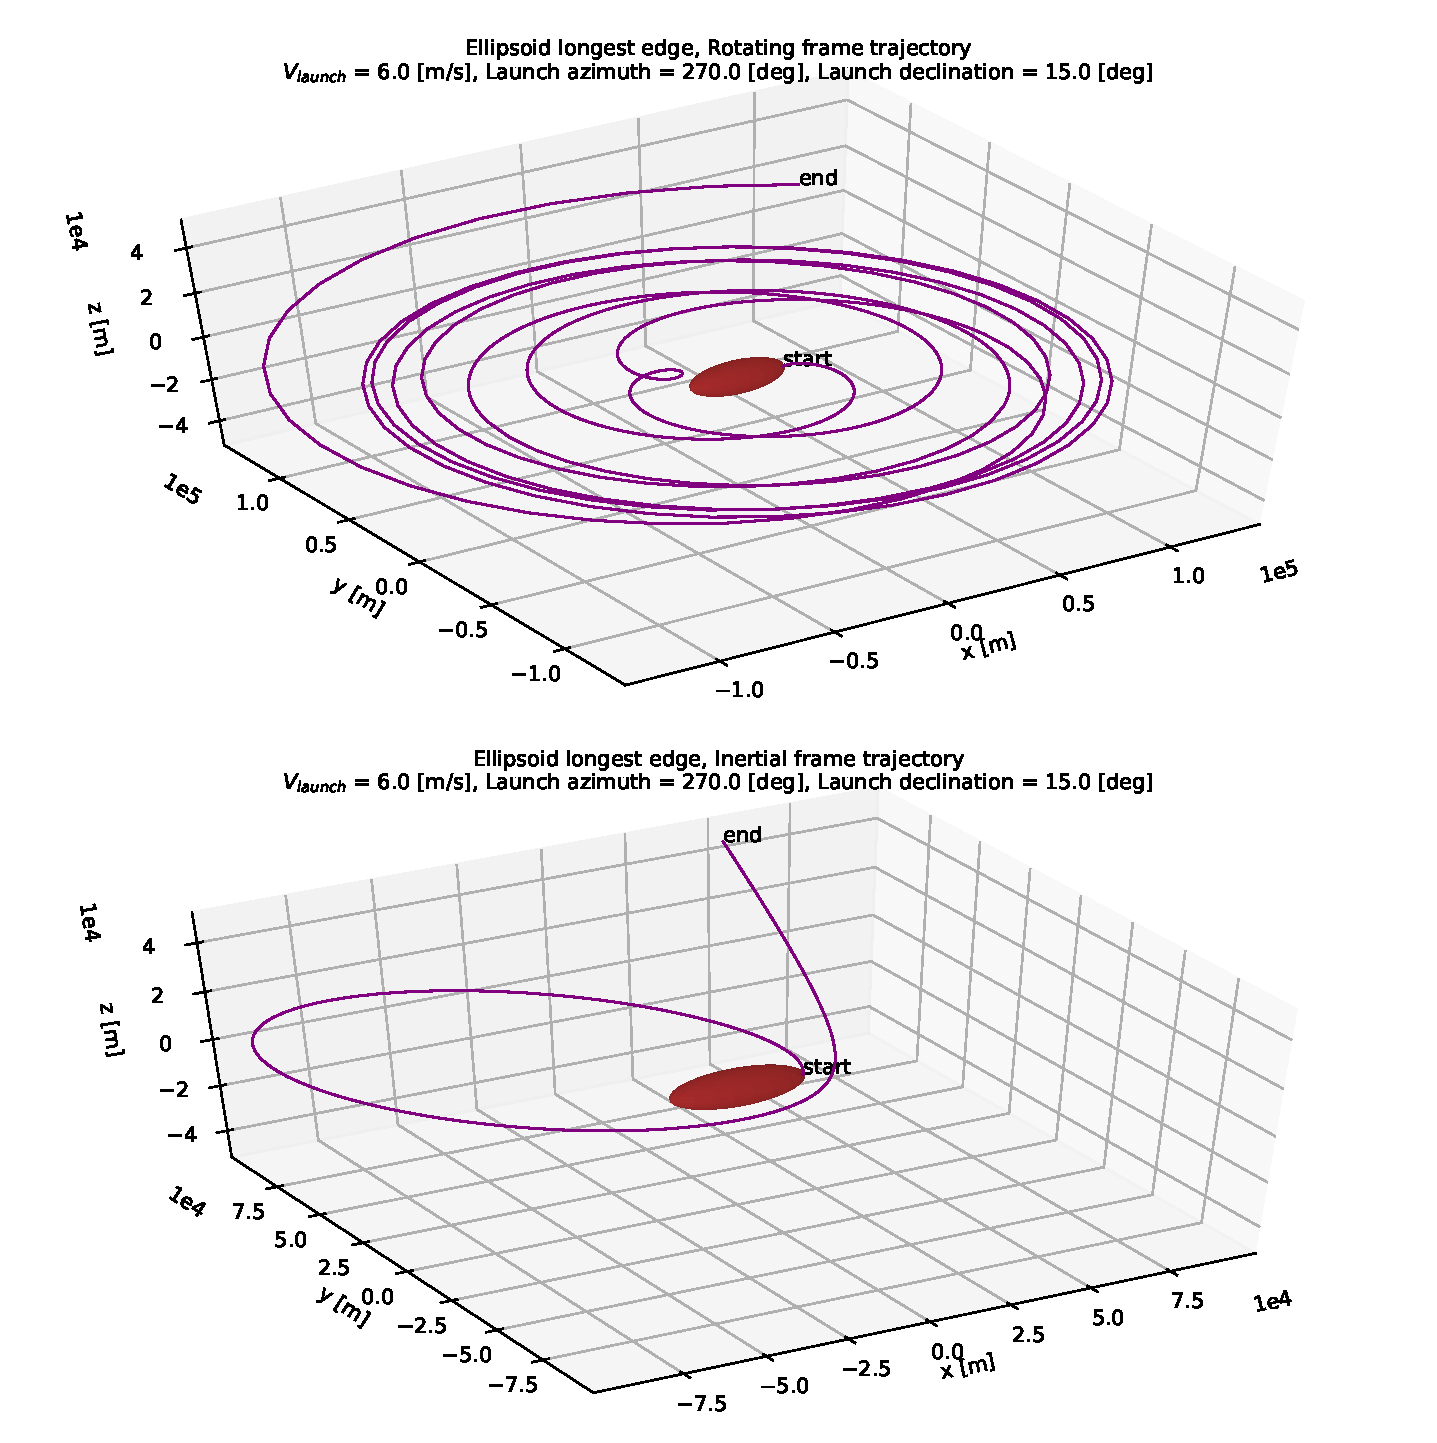
\includegraphics[width=\textwidth, height=0.7\textheight, keepaspectratio=true]{non_conservative_escape_speed/multiRev_3D_trajectory_declination15.pdf}
\caption{3D trajectory in the \gls{ARF} and the \gls{AIF} for launch declination angle \SI{15}{\degree} from \Cref{fig:non_conservative_escape_multiple_qinfinity_single_velocity}.}
\label{fig:3d_traj_declination_15}
\end{figure}
\FloatBarrier
%%%
The animation for the trajectory in \Cref{fig:3d_traj_declination_15} can be found at the web-link given in \Cref{fig:declination_15_animation}. The animation clearly shows the rapid rotation rate of the asteroid which accelerates the particle as it approaches behind it and completes the one and only revolution around the asteroid; having its velocity increased enough to eventually attain a positive energy and escape the asteroid. Thus with the help of gravity perturbations and a fast rotating asteroid, the particle changes from an elliptical orbit to a hyperbolic trajectory leading to its escape. This behavior can not be easily captured just from the initial conditions, as we observed, by the conservative guaranteed escape speed algorithm.
%
\newline\newline
%
An important thing to note here is that the initial condition of the regolith was such that its osculating eccentricity was above 1.0 (but a negative total energy), meaning that at the moment of the launch the regolith was on a hyperbolic trajectory but instantly evolves its orbit into an elliptical one. The reason for this is again the perturbations from a non-uniform gravity field and a rapidly rotating asteroid which keeps osculating the orbit. On the other hand, when we consider a spherical asteroid, the launched particle continues to propagate on the initial trajectory itself because in the absence of perturbations the initial orbital elements do not osculate. Thus for a spherical asteroid, a particle can only escape if the initial orbital elements are such that it is on a parabolic or a hyperbolic trajectory and not otherwise due to a lack of external influences to osculate the orbit. This is why the conservative guaranteed escape speed algorithm works for the spherical asteroid in predetermination of escape situations.
%%%
\begin{figure}[htb]
\centering
\captionsetup{justification=centering}

\includegraphics[width=\textwidth, height=0.1\textheight, keepaspectratio=true]{non_conservative_escape_speed/declination_15_animation.png}
\caption{Scan the QR code to view the 2D trajectory animation in the \gls{AIF} for launch declination angle \SI{15}{\degree} from \Cref{fig:non_conservative_escape_multiple_qinfinity_single_velocity}. The video can also be accessed from the following web-link: \url{https://youtu.be/5l_CAYnjotk}.}
\label{fig:declination_15_animation}
\end{figure}
\FloatBarrier
%%%
%%%
\begin{figure}[htb]
\centering
\captionsetup{justification=centering}
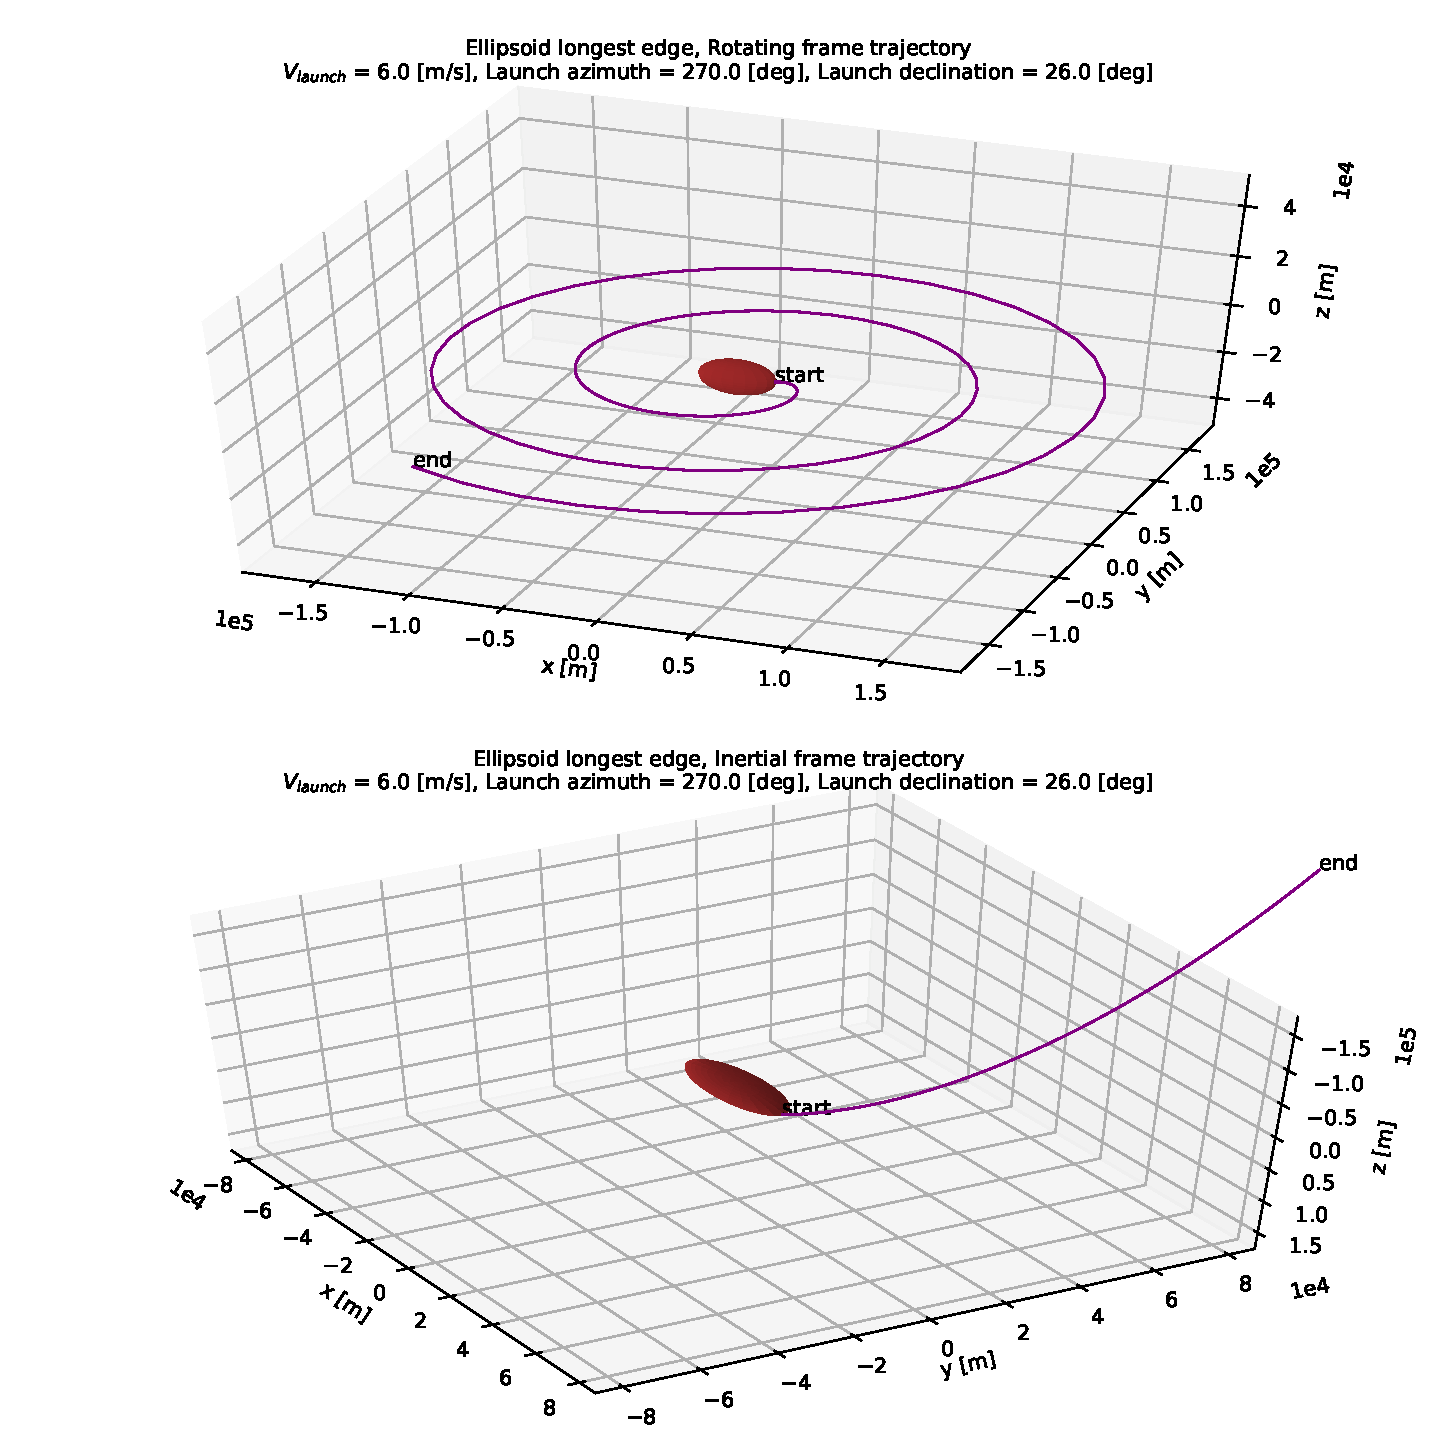
\includegraphics[width=\textwidth, height=0.55\textheight, keepaspectratio=true]{non_conservative_escape_speed/directEscape_3D_trajectory_declination26.pdf}
\caption{3D trajectory expressed in the \gls{ARF} and the \gls{AIF} for a launch declination angle of \SI{26}{\degree} from the normal direction. The particle launch conditions are the same as that used for \protect\Cref{fig:non_conservative_escape_multiple_qinfinity_single_velocity}.}
\label{fig:3d_traj_declination_26}
\end{figure}
\FloatBarrier
%%%
The final aspect that will be discussed in regard to the conservative guaranteed escape speed algorithm is its capacity to distinguish between particles that escape immediately and the ones that take one or more revolutions before escaping, when launched from an irregular body \parencite{scheeres2002fate}. However, we found out that this is only true if the particle is launched from the surface in the normal direction. In that, if the launch speed is lower than the conservative guaranteed escape speed and the particle escapes, then it underwent multiple revolutions. This was observed for multiple particles launched from the longest edge of the \gls{CDE} for launch velocities ranging from 1 to \SI{16}{\metre \per \second}. However, this phenomenon is not observed when the launch direction is not in the normal direction. For example, from \Cref{fig:non_conservative_escape_multiple_qinfinity_single_velocity}, the launch declination angle of \SI{26}{\degree} results in a direct escape scenario, even though the launch velocity is below the conservative guaranteed escape speed algorithm. The 3D trajectory for this case is shown in \Cref{fig:3d_traj_declination_26}.
%
\newline\newline
%
Thus, it is imperative to understand that with just a non-uniform gravity field and a relatively fast rotating asteroid, the dynamics for orbiting regolith become intangible enough such that predetermination of orbital behavior and final fate of the regolith can not be explained by simple analytical methods. We attempted to explain the complex behavior by deriving a different guaranteed escape speed algorithm, however, the method failed completely. We realize now that a numerical simulation method is a relatively better approach to understand the orbital dynamics of regolith lofted from an asteroid.

